\documentclass[tikz,border=5mm]{standalone}
\usepackage[T1]{fontenc}
\usepackage{lmodern}
\usetikzlibrary{arrows.meta}
\renewcommand{\familydefault}{\sfdefault}
% Green has one meaning: an accepted cut and its exported segment.
\definecolor{accepted}{HTML}{2C6B57}
\definecolor{acceptfill}{HTML}{EEF5F1}
\begin{document}
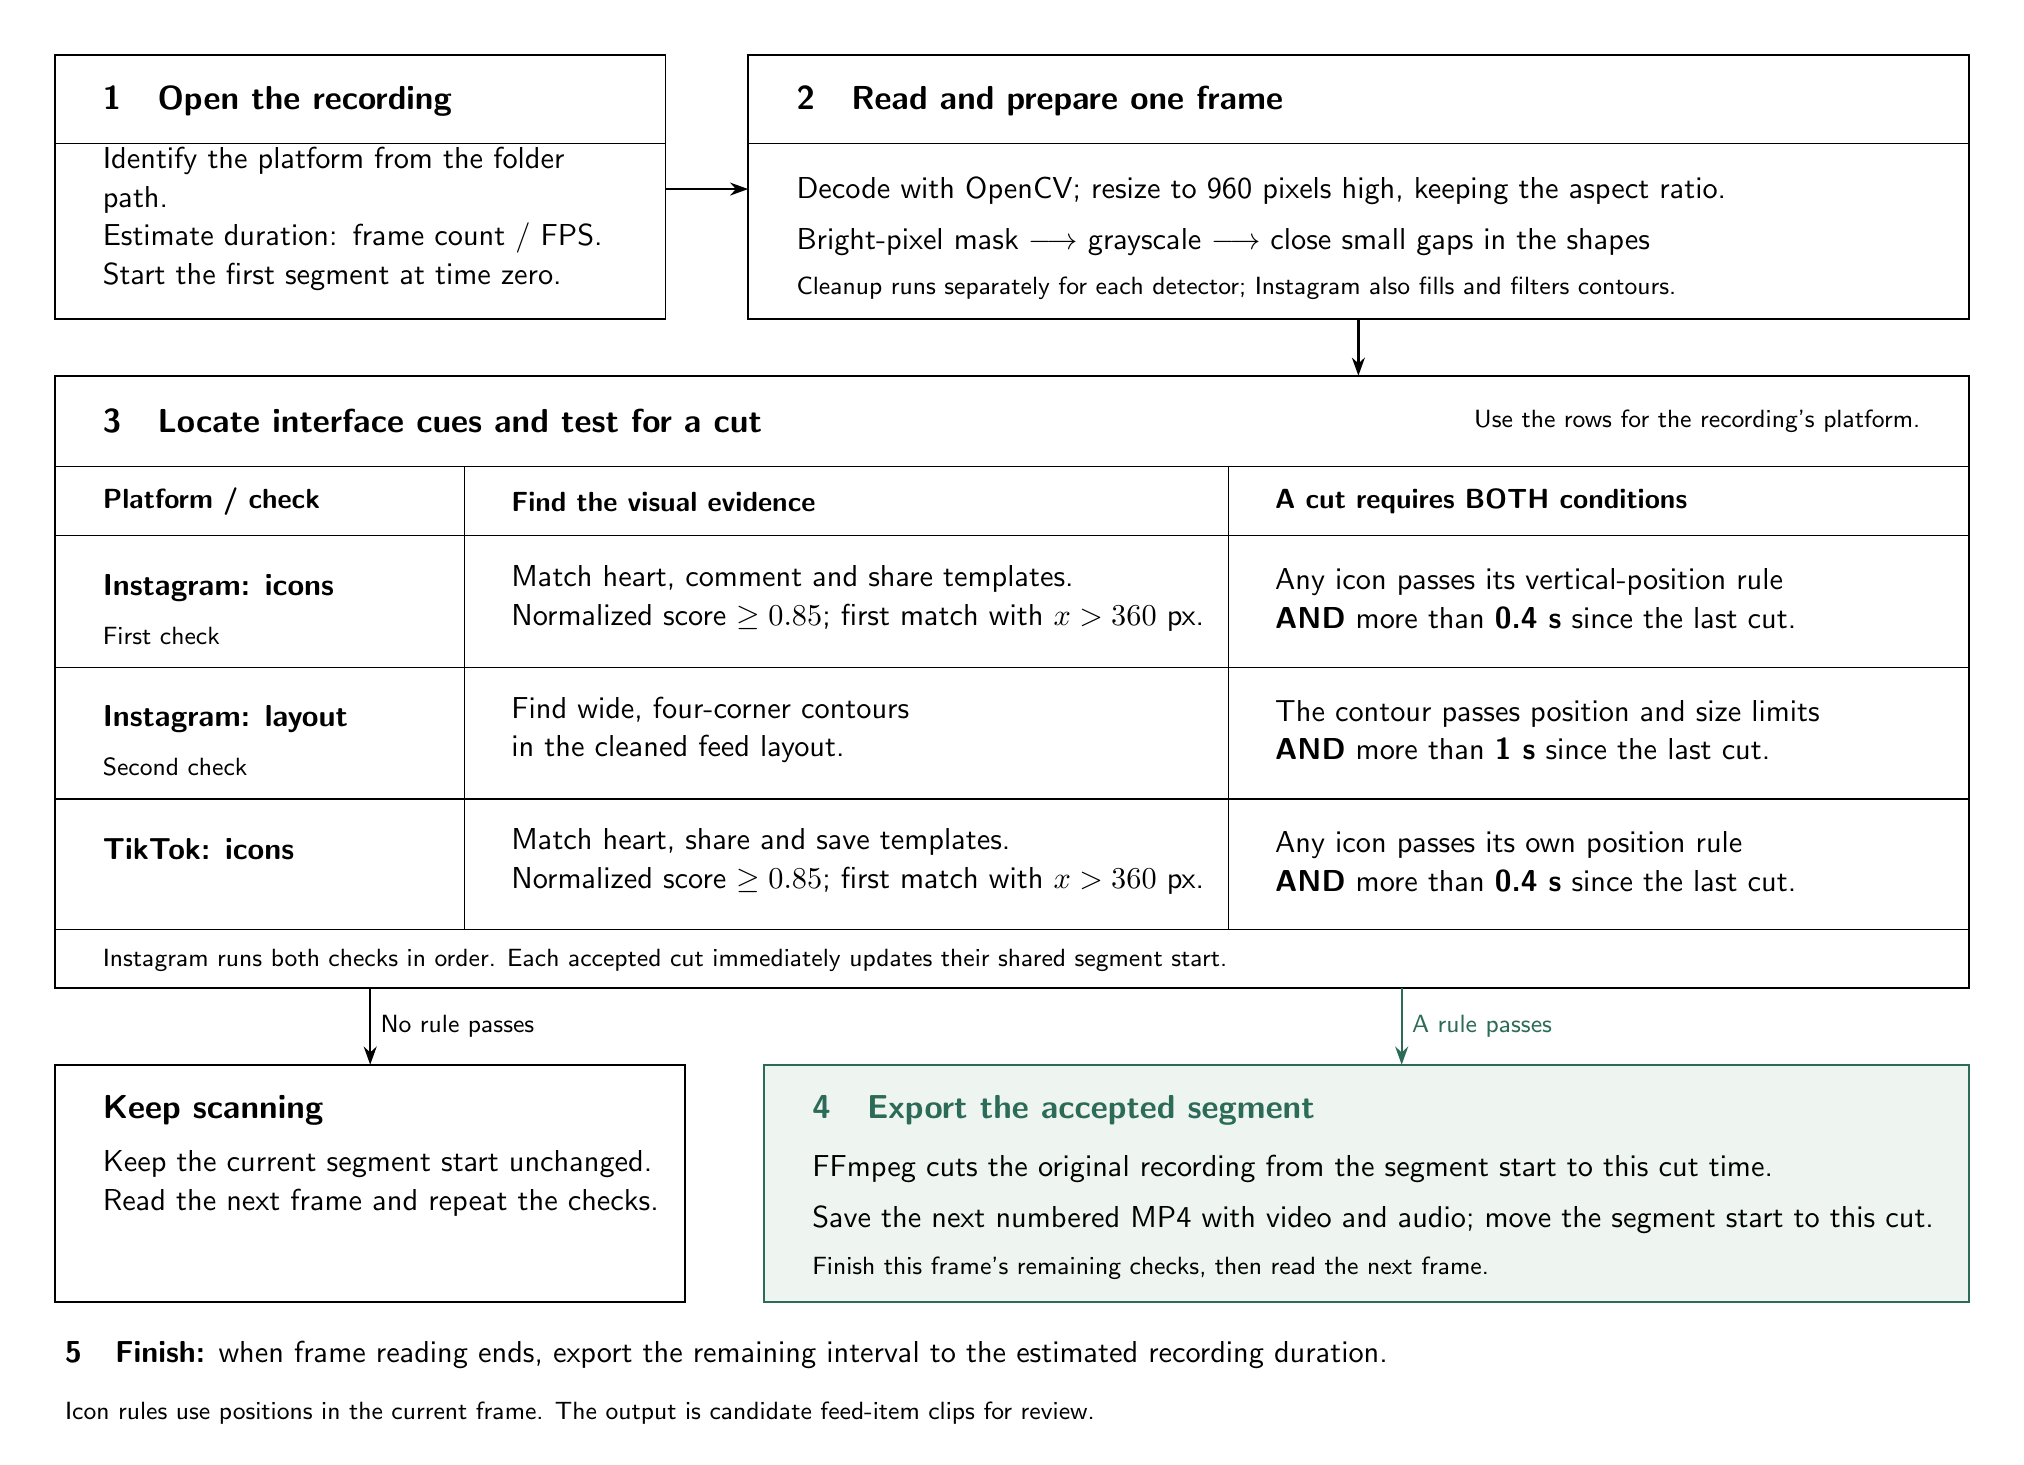
\begin{tikzpicture}[x=1cm,y=1cm,font=\sffamily,text=black,
  flow/.style={-{Stealth[length=2.3mm,width=1.65mm]},line width=.8pt},
  box/.style={draw=black,fill=white,line width=.65pt},
  heading/.style={font=\bfseries\fontsize{12}{15}\selectfont,align=left},
  body/.style={font=\fontsize{10.5}{14}\selectfont,align=left},
  note/.style={font=\fontsize{9.5}{12.5}\selectfont,align=left},
  column/.style={font=\bfseries\fontsize{10}{13}\selectfont,align=left}]
\useasboundingbox (0,0) rectangle (25,17.9);
\fill[white] (0,0) rectangle (25,17.9);

% SETUP AND PER-FRAME PREPARATION
\draw[box] (.35,14.20) rectangle (8.10,17.55);
\node[heading,anchor=west] at (.83,16.96) {1\quad Open the recording};
\draw[line width=.4pt] (.35,16.43)--(8.10,16.43);
\node[body,anchor=west,text width=6.75cm] at (.83,15.47)
  {Identify the platform from the folder path.\\Estimate duration: frame count / FPS.\\Start the first segment at time zero.};

\draw[box] (9.15,14.20) rectangle (24.65,17.55);
\node[heading,anchor=west] at (9.64,16.96) {2\quad Read and prepare one frame};
\draw[line width=.4pt] (9.15,16.43)--(24.65,16.43);
\node[body,anchor=west] at (9.64,15.83)
  {Decode with OpenCV; resize to 960 pixels high, keeping the aspect ratio.};
\node[body,anchor=west] at (9.64,15.18)
  {Bright-pixel mask $\longrightarrow$ grayscale $\longrightarrow$ close small gaps in the shapes};
\node[note,anchor=west] at (9.64,14.59)
  {Cleanup runs separately for each detector; Instagram also fills and filters contours.};
\draw[flow] (8.10,15.85)--(9.15,15.85);
\draw[flow] (16.90,14.20)--(16.90,13.48);

% THE METHOD: SAME FRAME, PLATFORM-SPECIFIC EVIDENCE AND ACCEPTANCE RULES
\draw[box] (.35,5.70) rectangle (24.65,13.48);
\node[heading,anchor=west] at (.83,12.90) {3\quad Locate interface cues and test for a cut};
\node[note,anchor=east] at (24.16,12.90) {Use the rows for the recording's platform.};
\draw[line width=.45pt] (.35,12.33)--(24.65,12.33);
\node[column,anchor=west] at (.83,11.88) {Platform / check};
\node[column,anchor=west] at (6.02,11.88) {Find the visual evidence};
\node[column,anchor=west] at (15.72,11.88) {A cut requires BOTH conditions};
\draw[line width=.4pt] (.35,11.45)--(24.65,11.45);
\draw[line width=.4pt] (5.55,6.45)--(5.55,12.33);
\draw[line width=.4pt] (15.25,6.45)--(15.25,12.33);

% Instagram icon rule, first on each Instagram frame.
\node[body,anchor=west,font=\bfseries\fontsize{11}{14}\selectfont] at (.83,10.79) {Instagram: icons};
\node[note,anchor=west] at (.83,10.17) {First check};
\node[body,anchor=west] at (6.02,10.65)
  {Match heart, comment and share templates.\\Normalized score $\geq 0.85$; first match with $x>360$ px.};
\node[body,anchor=west] at (15.72,10.65)
  {Any icon passes its vertical-position rule\\\textbf{AND} more than \textbf{0.4 s} since the last cut.};
\draw[line width=.35pt] (.35,9.77)--(24.65,9.77);

% Instagram layout rule follows the icon rule; this is not a content classifier.
\node[body,anchor=west,font=\bfseries\fontsize{11}{14}\selectfont] at (.83,9.12) {Instagram: layout};
\node[note,anchor=west] at (.83,8.51) {Second check};
\node[body,anchor=west] at (6.02,8.98)
  {Find wide, four-corner contours\\in the cleaned feed layout.};
\node[body,anchor=west] at (15.72,8.98)
  {The contour passes position and size limits\\\textbf{AND} more than \textbf{1 s} since the last cut.};
\draw[line width=.65pt] (.35,8.10)--(24.65,8.10);

% TikTok uses its own templates and per-icon position thresholds.
\node[body,anchor=west,font=\bfseries\fontsize{11}{14}\selectfont] at (.83,7.47) {TikTok: icons};
\node[body,anchor=west] at (6.02,7.31)
  {Match heart, share and save templates.\\Normalized score $\geq 0.85$; first match with $x>360$ px.};
\node[body,anchor=west] at (15.72,7.31)
  {Any icon passes its own position rule\\\textbf{AND} more than \textbf{0.4 s} since the last cut.};
\draw[line width=.4pt] (.35,6.45)--(24.65,6.45);
\node[note,anchor=west] at (.83,6.06)
  {Instagram runs both checks in order. Each accepted cut immediately updates their shared segment start.};

% THE TWO OUTCOMES: SAME NEXT FRAME, DIFFERENT SEGMENT START
\draw[flow] (4.35,5.70)--node[right,note] {No rule passes} (4.35,4.73);
\draw[flow,draw=accepted] (17.45,5.70)--node[right,note,text=accepted] {A rule passes} (17.45,4.73);
\draw[box] (.35,1.72) rectangle (8.35,4.73);
\node[heading,anchor=west] at (.83,4.15) {Keep scanning};
\node[body,anchor=west] at (.83,3.22)
  {Keep the current segment start unchanged.\\Read the next frame and repeat the checks.};

\draw[draw=accepted,fill=acceptfill,line width=.8pt] (9.35,1.72) rectangle (24.65,4.73);
\node[heading,anchor=west,text=accepted] at (9.84,4.15) {4\quad Export the accepted segment};
\node[body,anchor=west] at (9.84,3.40)
  {FFmpeg cuts the original recording from the segment start to this cut time.};
\node[body,anchor=west] at (9.84,2.76)
  {Save the next numbered MP4 with video and audio; move the segment start to this cut.};
\node[note,anchor=west] at (9.84,2.15)
  {Finish this frame's remaining checks, then read the next frame.};

% TERMINATION AND INTERPRETATION, KEPT OUTSIDE THE MAIN DECISION TABLE
\node[body,anchor=west] at (.35,1.04)
  {\textbf{5\quad Finish:} when frame reading ends, export the remaining interval to the estimated recording duration.};
\node[note,anchor=west] at (.35,.30) {Icon rules use positions in the current frame. The output is candidate feed-item clips for review.};
\end{tikzpicture}
\end{document}
